\documentclass{article}
\usepackage[a4paper, total={6in, 9in}]{geometry}

\usepackage[utf8]{inputenc}
\usepackage{graphicx}
\graphicspath{ {./images/} }
\usepackage{float}
\usepackage{circuitikz}
\usepackage{etoolbox}
\makeatletter
\providecommand{\subtitle}[1]{% add subtitle to \maketitle
  \apptocmd{\@title}{\par {\large #1}}{}{}
}
\makeatother


\title{
\includegraphics[scale=0.65]{images/ozu.png}\\
\textbf{EE202 - Circuit Analysis}}
\subtitle{Laboratory #5}
\date{Fall 2022}
%\author{Laboratory 1}

\newcommand{\HRule}{\rule{\linewidth}{0.5mm}}

\begin{document}

\begin{titlepage}
\begin{center}

% Top 

\includegraphics[width=0.55\textwidth]{ozu.png}~\\[2cm]

% Title
\HRule \\[0.4cm]
{ \LARGE 
  \textbf{Lab Report for EE202 Circuit Analysis}\\[0.4cm]
  \emph{Laboratory 5}\\[0.4cm]
}
\HRule \\[1.5cm]

% Author
{ \large
  Ömer Faruk Avcı \\[0.1cm]
  \texttt{faruk.avci@ozu.edu.tr}
}

\vfill

%\textsc{\Large Cyprus University of Technology}\\[0.4cm]
\textsc{\large Department of Electrical and Electronics Engineering}\\[0.4cm]


% Bottom
{\large \today}
 
\end{center}
\end{titlepage}



\newpage

%\maketitle

\section{Introduction}
The purpose of this lab is to introduce first-order circuits and see the use of a first-order circuit in a practical oscillator circuit. The lab involves analyzing a first-order RC circuit, simulating it using SPICE, and designing a timer circuit using the LM555 IC to create a blinking LED with a specific time period.


\subsection{Preliminary Work}
\subsubsection{PreTask 1}



\begin{figure}[h]
  \centering
  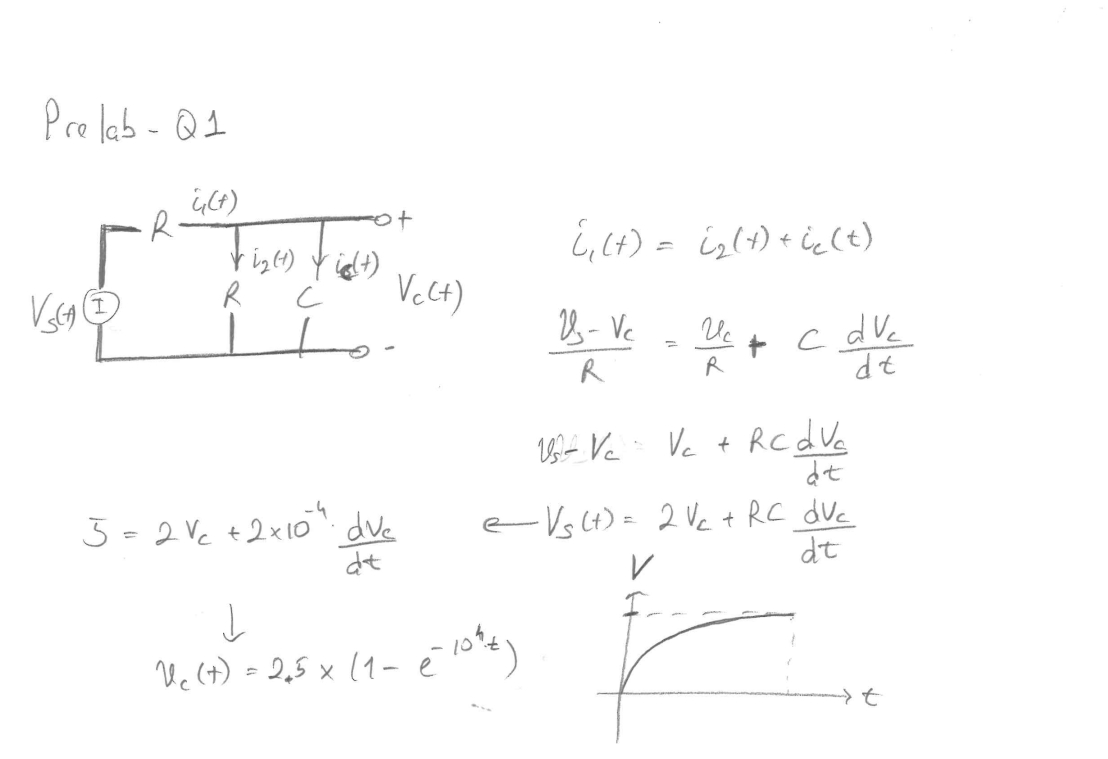
\includegraphics[scale=0.4]{prelab-task1.png}
  \caption{Pre-lab Task 1 Solution}
\end{figure}


\newpage
\subsubsection{PreTask 2}

\begin{figure}[h]
  
  \centering
  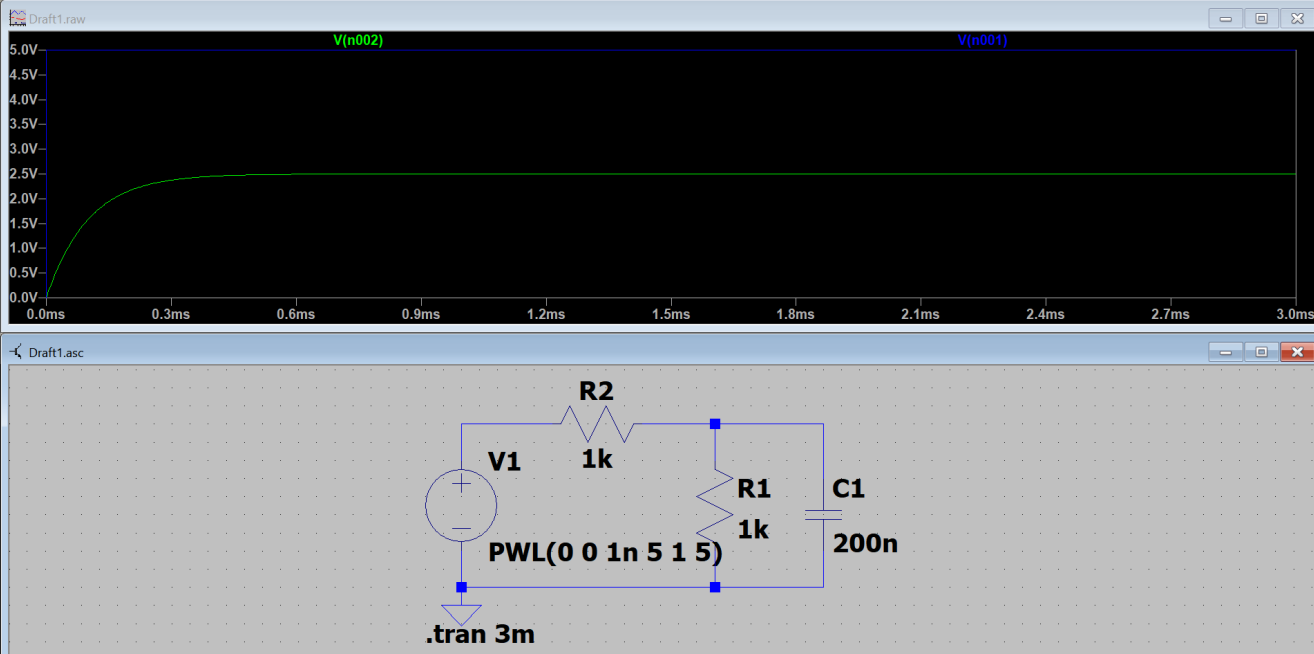
\includegraphics[scale=0.3]{prelab-task2.png}
  \caption{Pre-lab Task 2 LTSpice Results}
\end{figure}




\subsubsection{PreTask 3}





\begin{figure}[h]
  \centering
  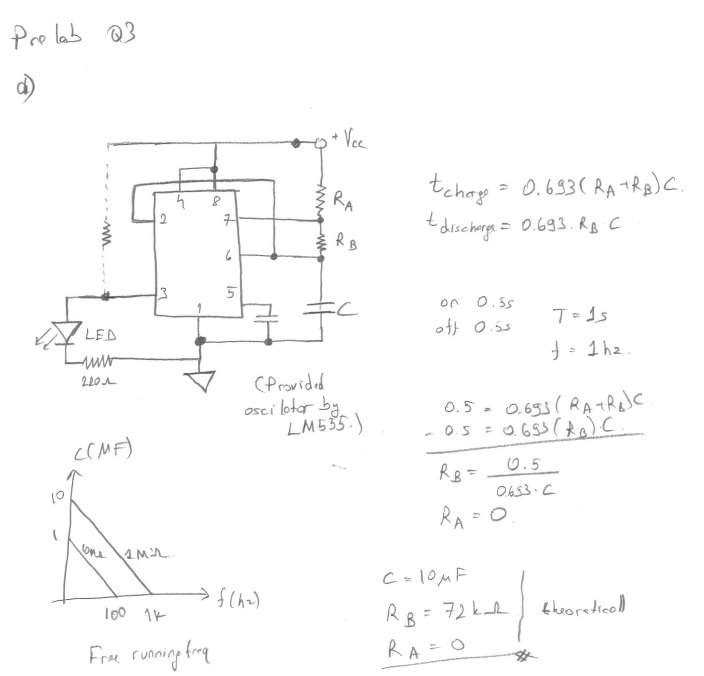
\includegraphics[scale=0.351]{prelab-task3-a.png}
  \caption{Pre-lab Task 3 Part 1 Solution}
\end{figure}



\newpage

\begin{figure}[h]
  
  \centering
  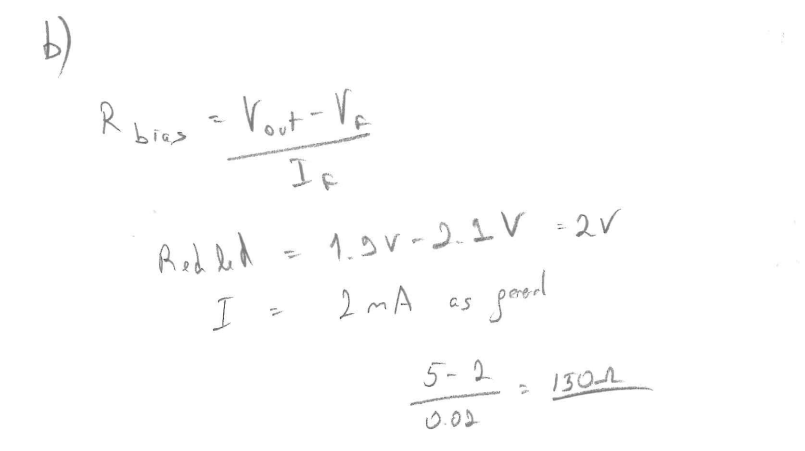
\includegraphics[scale=0.5]{prelab-task3-b.png}
  \caption{Pre-lab Task 3 Part 2 Solution}
\end{figure}






\subsection{Lab Tasks}
\subsubsection{Task 1: First Order Circuit}
Task 1 is about constructing the RC circuit analyzed in the preliminary work Figure 1 and observing
the capacitor voltage’s waveform change depending on the frequency.

\noindent
The circuit is constructed using standard components, including 1k Ohm resistors and 200nF capacitors.

\begin{figure}[h]
  \centering
  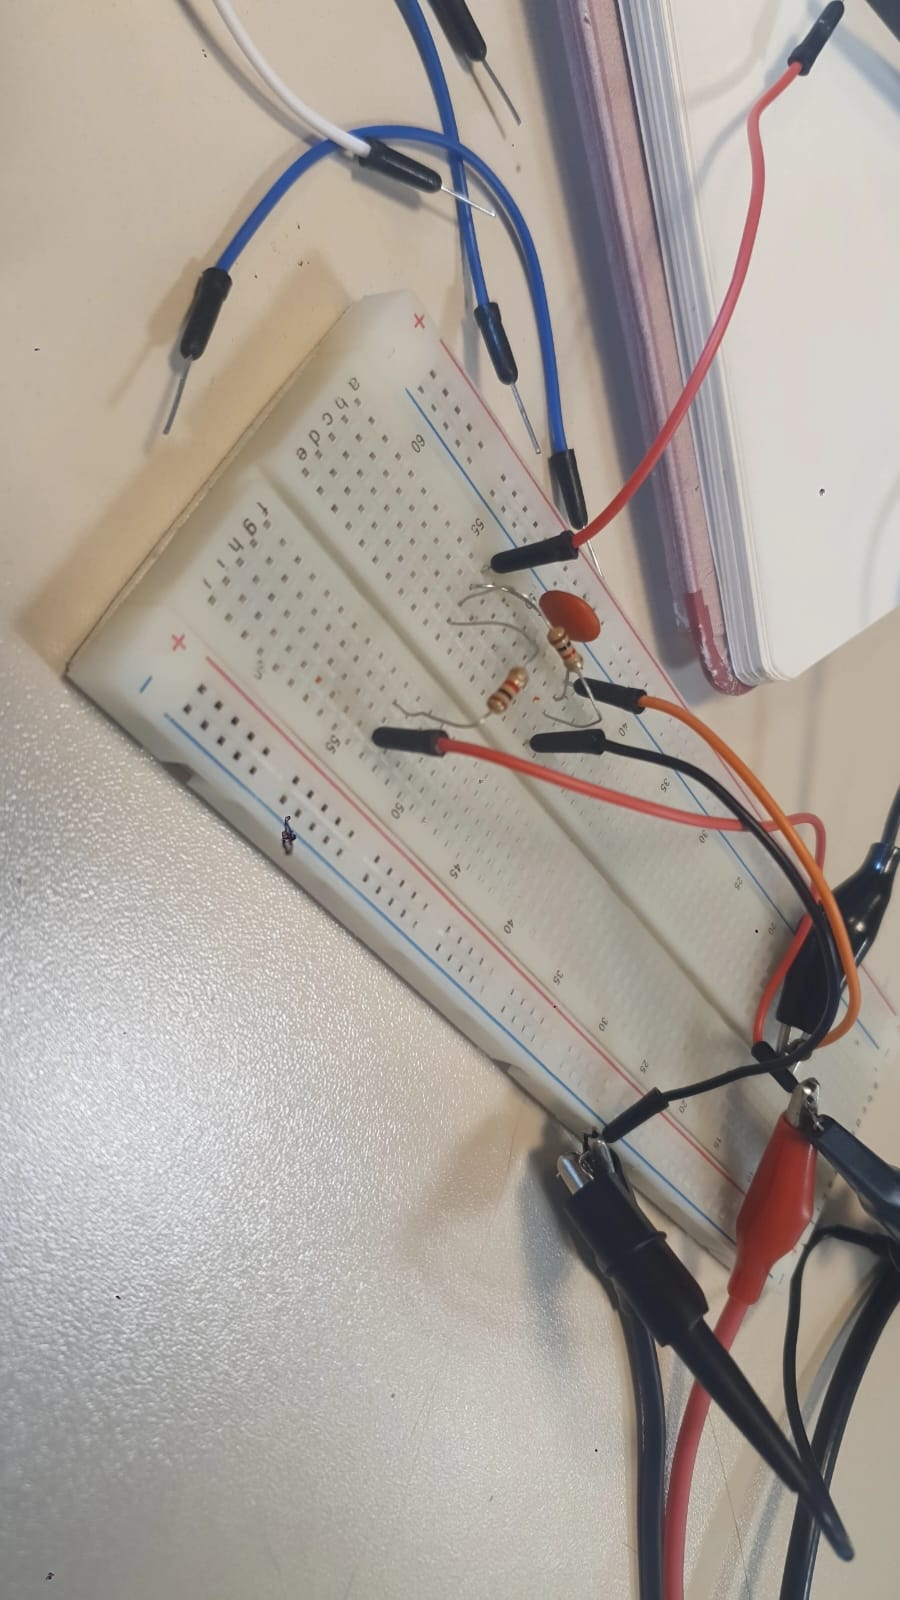
\includegraphics[scale=0.2, angle=90]{task1-circuit.png}
  \caption{Circuit Diagram for Task 1}
\end{figure}
\newpage

\noindent
The function generator was set to output a 5V square wave with a period of 2 ms, ensuring the half period was more than 10 times the time constant of the circuit. The voltage over the capacitor was observed on the oscilloscope, and the resulting waveform was captured and included in the report. Results from the oscilloscope can be seen as follows:
\begin{figure}[h]
  \centering
  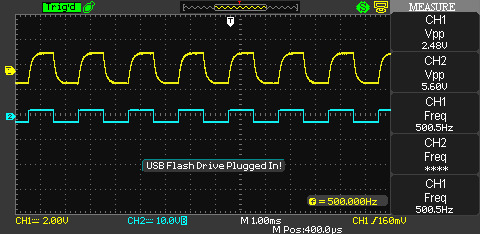
\includegraphics[scale=0.8]{ADS00003.jpg}
  \caption{Output Signal for T = 2ms}
\end{figure}

The frequency of the square wave was increased to observe the RC circuit's response. Results are:
\begin{figure}[h]
  \centering
  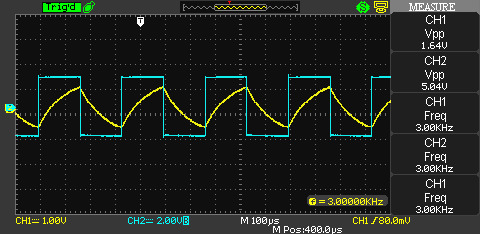
\includegraphics[scale=0.8]{ADS00006.jpg}
  \caption{Output Signal for f = 3kHz}
\end{figure} 

\noindent
\textbf{Comments: }Yellow-colored signals (Ch1) represent the output, while blue-colored waveforms (Ch2) represent the input. It is clearly seen that as the frequency of the input signal increases (i.e., the period decreases), the output signal transitions from a more defined waveform to a ramp-like shape with reduced amplitude.



\newpage


\subsubsection{Task 2: Timer Circuit}

In this task, an LED-flashing first-order RC oscillator circuit is built using an LM555 timer. The circuit converts the DC input from the power supply into a square-wave AC output with a frequency around 1Hz. The LED flashes in sync with the output pulses, demonstrating that Vout is a periodic AC signal.


\begin{figure}[h]
  \centering
  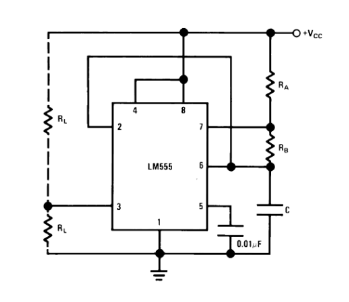
\includegraphics[scale=0.5]{task2-diagram.png}
  \caption{Oscillator Circuit Diagram}
\end{figure}

\noindent
The circuit is built using the LM555 timer with appropriate pin connections and carefully selected resistor and capacitor values to achieve the desired frequency (~1Hz) and duty cycle.

\begin{figure}[h]
    \centering
    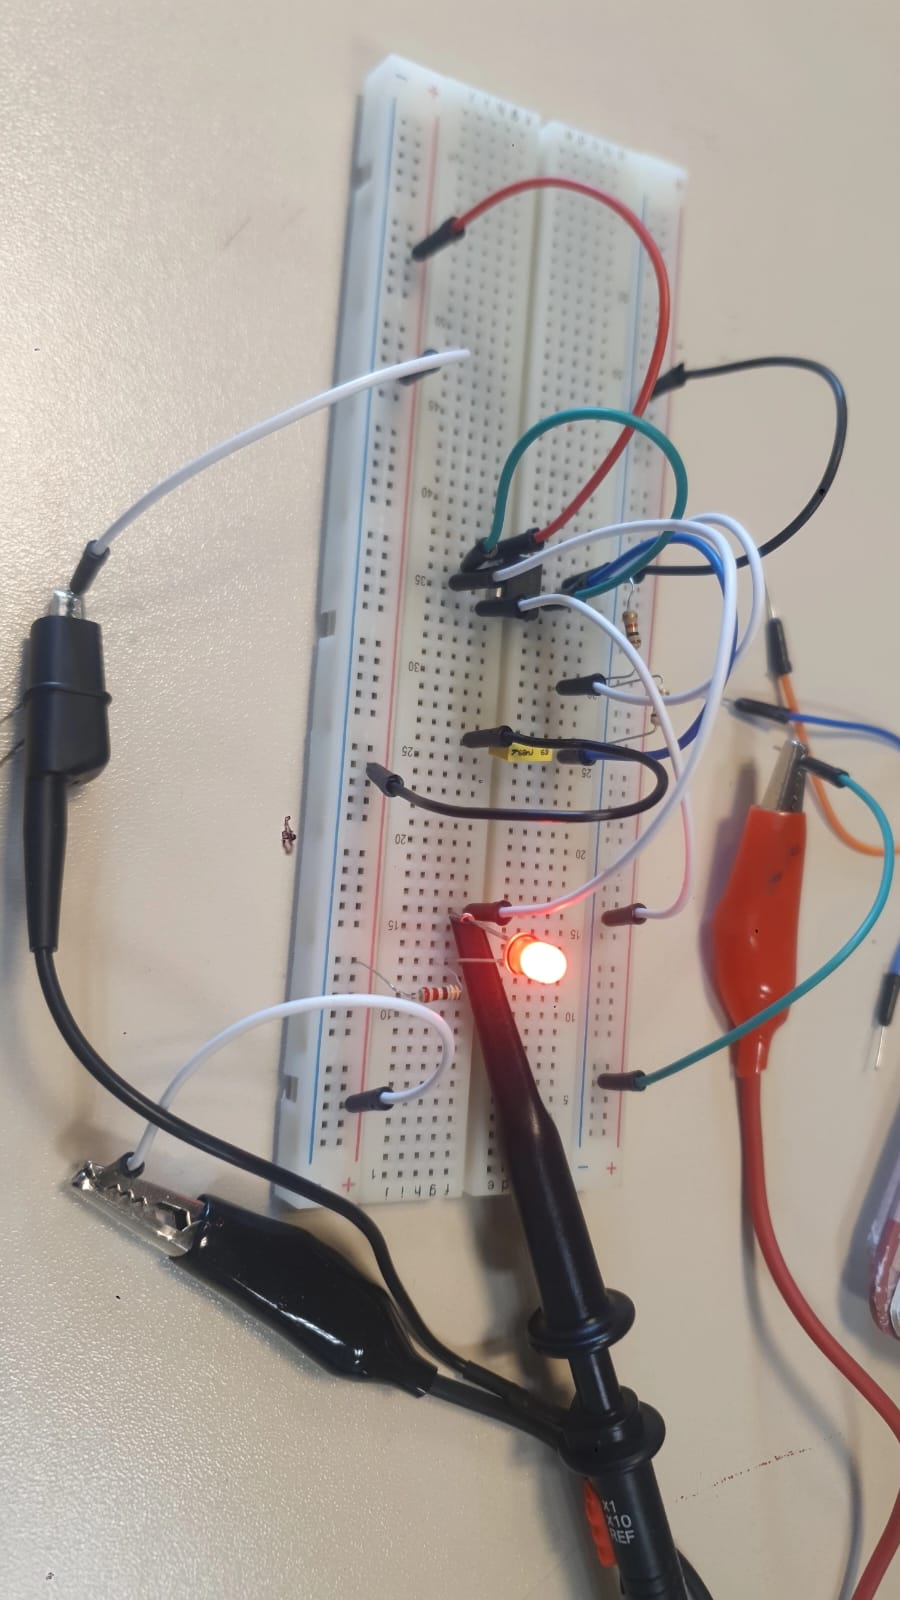
\includegraphics[scale=0.25 ,angle=90]{task2-circuit.png}
    \caption{LED-Flashing Timer Circuit}
\end{figure}

Due to limited resistor availability, we used megaohm-range resistors for RA and RB. After adjusting with the closest values we had, the LED started flashing at around 1Hz. The output waveform was confirmed on the oscilloscope, and minor tuning was done to approach a 1-second period. Oscillator results can be seen as follows:

\begin{figure}
  \centering

  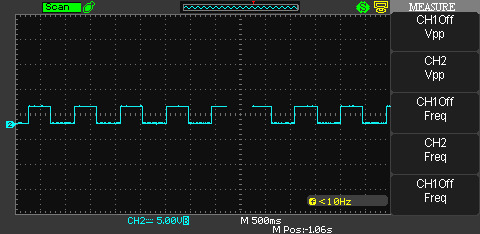
\includegraphics[scale=0.8]{ADS00007.jpg}
  \caption{Oscillator Output Waveform}
\end{figure}

\section{Conclusion}
\subsubsection{Task 1.}
In this lab, we explored the behavior of RC circuits and the LM555 timer. For Task 1, we observed how increasing frequency caused the output voltage (Vout) to decrease due to reduced capacitive reactance, while the input voltage (Vin) remained unaffected. The waveforms supported the theoretical understanding of capacitor charge/discharge dynamics.

\subsubsection{Task 2.}
In Task 2, we constructed a timer circuit using the LM555. Due to resistor availability, we used high-value resistors to achieve near 1Hz flashing. The output signal and LED flashing matched expectations, confirming our adjustments were effective. Overall, the lab helped reinforce the theory through hands-on experience with timing circuits and waveform behavior.

\noindent
Minor deviations—such as a measured frequency of 1.24 Hz instead of the expected 1 Hz—can be attributed to component tolerances, oscilloscope precision limits, and wiring or breadboard imperfections. These small errors (typically within 10–20\%) are normal and did not significantly affect overall results.


\end{document}
